%%
%% This is file `sample-sigconf.tex',
%% generated with the docstrip utility.
%%
%% The original source files were:
%%
%% samples.dtx  (with options: `sigconf')
%% 
%% IMPORTANT NOTICE:
%% 
%% For the copyright see the source file.
%% 
%% Any modified versions of this file must be renamed
%% with new filenames distinct from sample-sigconf.tex.
%% 
%% For distribution of the original source see the terms
%% for copying and modification in the file samples.dtx.
%% 
%% This generated file may be distributed as long as the
%% original source files, as listed above, are part of the
%% same distribution. (The sources need not necessarily be
%% in the same archive or directory.)
%%
%% The first command in your LaTeX source must be the \documentclass command.
\documentclass[sigconf]{acmart}
\settopmatter{printacmref=false, printccs=true, printfolios=true}
%%
%% \BibTeX command to typeset BibTeX logo in the docs
\AtBeginDocument{%
	\providecommand\BibTeX{{%
			\normalfont B\kern-0.5em{\scshape i\kern-0.25em b}\kern-0.8em\TeX}}}

%% Rights management information.  This information is sent to you
%% when you complete the rights form.  These commands have SAMPLE
%% values in them; it is your responsibility as an author to replace
%% the commands and values with those provided to you when you
%% complete the rights form.
%\setcopyright{acmcopyright}
%\copyrightyear{2018}
%\acmYear{2018}
%\acmDOI{10.1145/1122445.1122456}

%% These commands are for a PROCEEDINGS abstract or paper.
%\acmConference[Woodstock '18]{Woodstock '18: ACM Symposium on Neural
%	Gaze Detection}{June 03--05, 2018}{Woodstock, NY}
%\acmBooktitle{Woodstock '18: ACM Symposium on Neural Gaze Detection,
%	June 03--05, 2018, Woodstock, NY}
%\acmPrice{15.00}
%\acmISBN{978-1-4503-XXXX-X/18/06}


%%
%% Submission ID.
%% Use this when submitting an article to a sponsored event. You'll
%% receive a unique submission ID from the organizers
%% of the event, and this ID should be used as the parameter to this command.
%%\acmSubmissionID{123-A56-BU3}

%%
%% The majority of ACM publications use numbered citations and
%% references.  The command \citestyle{authoryear} switches to the
%% "author year" style.
%%
%% If you are preparing content for an event
%% sponsored by ACM SIGGRAPH, you must use the "author year" style of
%% citations and references.
%% Uncommenting
%% the next command will enable that style.
%%\citestyle{acmauthoryear}
\usepackage{xspace}
\newcommand{\etal}{\textit{et al.}\xspace}
\newcommand{\ie}{\textit{i.e.,}\xspace}
\newcommand{\eg}{\textit{e.g.,}\xspace}
%%
%% end of the preamble, start of the body of the document source.
\begin{document}
	
	%%
	%% The "title" command has an optional parameter,
	%% allowing the author to define a "short title" to be used in page headers.
	\title{Opening sentences of research papers	}
	\subtitle{	How academics defeat the blinking cursor }
	
	%%
	%% The "author" command and its associated commands are used to define
	%% the authors and their affiliations.
	%% Of note is the shared affiliation of the first two authors, and the
	%% "authornote" and "authornotemark" commands
	%% used to denote shared contribution to the research.
	
	
	%%
	%% By default, the full list of authors will be used in the page
	%% headers. Often, this list is too long, and will overlap
	%% other information printed in the page headers. This command allows
	%% the author to define a more concise list
	%% of authors' names for this purpose.
	%\renewcommand{\shortauthors}{Trovato and Tobin, et al.}
	
	%%
	%% The abstract is a short summary of the work to be presented in the
	%% article.
	\begin{abstract}
		abstract
	\end{abstract}
	
	%%
	%% The code below is generated by the tool at http://dl.acm.org/ccs.cfm.
	%% Please copy and paste the code instead of the example below.
	%%
	\begin{CCSXML}
		<ccs2012>
		<concept>
		<concept_id>10010520.10010553.10010562</concept_id>
		<concept_desc>Computer systems organization~Embedded systems</concept_desc>
		<concept_significance>500</concept_significance>
		</concept>
		<concept>
		<concept_id>10010520.10010575.10010755</concept_id>
		<concept_desc>Computer systems organization~Redundancy</concept_desc>
		<concept_significance>300</concept_significance>
		</concept>
		<concept>
		<concept_id>10010520.10010553.10010554</concept_id>
		<concept_desc>Computer systems organization~Robotics</concept_desc>
		<concept_significance>100</concept_significance>
		</concept>
		<concept>
		<concept_id>10003033.10003083.10003095</concept_id>
		<concept_desc>Networks~Network reliability</concept_desc>
		<concept_significance>100</concept_significance>
		</concept>
		</ccs2012>
	\end{CCSXML}
	
	\ccsdesc[500]{xx}
	
	%%
	%% Keywords. The author(s) should pick words that accurately describe
	%% the work being presented. Separate the keywords with commas.
	\keywords{xx}
	
	%% A "teaser" image appears between the author and affiliation
	%% information and the body of the document, and typically spans the
	%% page.
	
	%%
	%% This command processes the author and affiliation and title
	%% information and builds the first part of the formatted document.
	\maketitle
	\section{Introduction}
	How do researchers start their papers? We wanted to understand how other researchers approach the opening sentence in their work. For this purpose, we studied three years of papers (379 papers in total) from USENIX Security, one of the top venues for security research. More pertinently, it is a venue with open access, easy-to-download full proceedings in a variety of friendly formats that made our job easier. We read every opening sentence from the main body of the paper (as opposed to the abstract). For this work, we drew inspiration from Grounded Theory~\cite{glaser1968discovery}---we applied coding for each sentence. After numerous iterations several patterns started to emerge and as a result, we developed and refined a detailed categorization for opening sentences. 
	
	% GITHUB Link???
	\section{Related Work}
	Different aspects of academic writing has been explored in the literature. King analyses opening sentences in medical research in his article~\cite{king1967opening}. He states that the opening sentence should draw readers' attention, and it should also be concise and clear about stating the main theme of the paper. He also gives examples from medical writing and explains different ways to simplify overcomplicated sentences by shortening them. Cameron \etal explains the struggles of the writing process and suggests strategies to helps novice writers to overcome them~\cite{cameron2009demystifying}. Hartley presents a bilingual study in English and Spanish on research papers in psychology~\cite{hartley2012new}. The paper focuses on improving different aspects of academic writing to increase readability. Biber \etal discuss the stereotypical characteristics of academic writing like complex grammar structures~\cite{biber2010challenging}.
	
	
	\section{Methodology}
	\subsection{Grounded theory}
	%What is grounded theory? How is it done theoretically? Which steps did we follow and how did we adapt?
	
	Grounded theory is a qualitative data analysis method~\cite{glaser1968discovery}. The collected qualitative data  (\eg interview transcripts) is sorted through qualitative coding. By performing coding, the aim is to come up with new high-level theories and concepts at the end of the process. Coding is an iterative process, as several rounds of coding can be performed to refine the categories. At the end of the process,  a new theory that is based on the data is presented.
	
	In this paper, we applied coding for each opening sentence. We created codes and labeled each sentence by these codes. We observed the relations among the codes to categorize them and we ended up with the categorization shown in Figure~\ref{fig:overview}.  We used coding to determine common patterns among opening sentences. 
	
	%coding :
	%Open Coding: The data is separated into parts, codes are created and each part is labeled by these codes.
	% Axial Coding:  Based on the relations observed among the codes, they are put into categories.
	% Selective Coding: The categories from the previous step are combined into a single, core category, that is the premise of the thesis of the research .
	
	
	Grounded Theory is also used as a methodology in security and privacy research. It is used to study user mental models of cryptocurrency systems~\cite{mai2020user}, how blockchain technology is perceived and how it is used~\cite{ruoti2019blockchain}, preferences for security warning types~\cite{danilova2020one}, the factors that influence software developers' motivation towards security~\cite{assal2018motivations},  how users manage their online security posture~\cite{ruoti2017weighing}, and how users manage their passwords~\cite{stobert2014password}.
	
	
	
	
	
	\section{Description of Each Category}
	We provide a description of each category Figure~\ref{fig:overview} show the hierarchy chart of the categories.
	
	\label{sec:categories}
	\begin{figure*}[t]
		\centering
		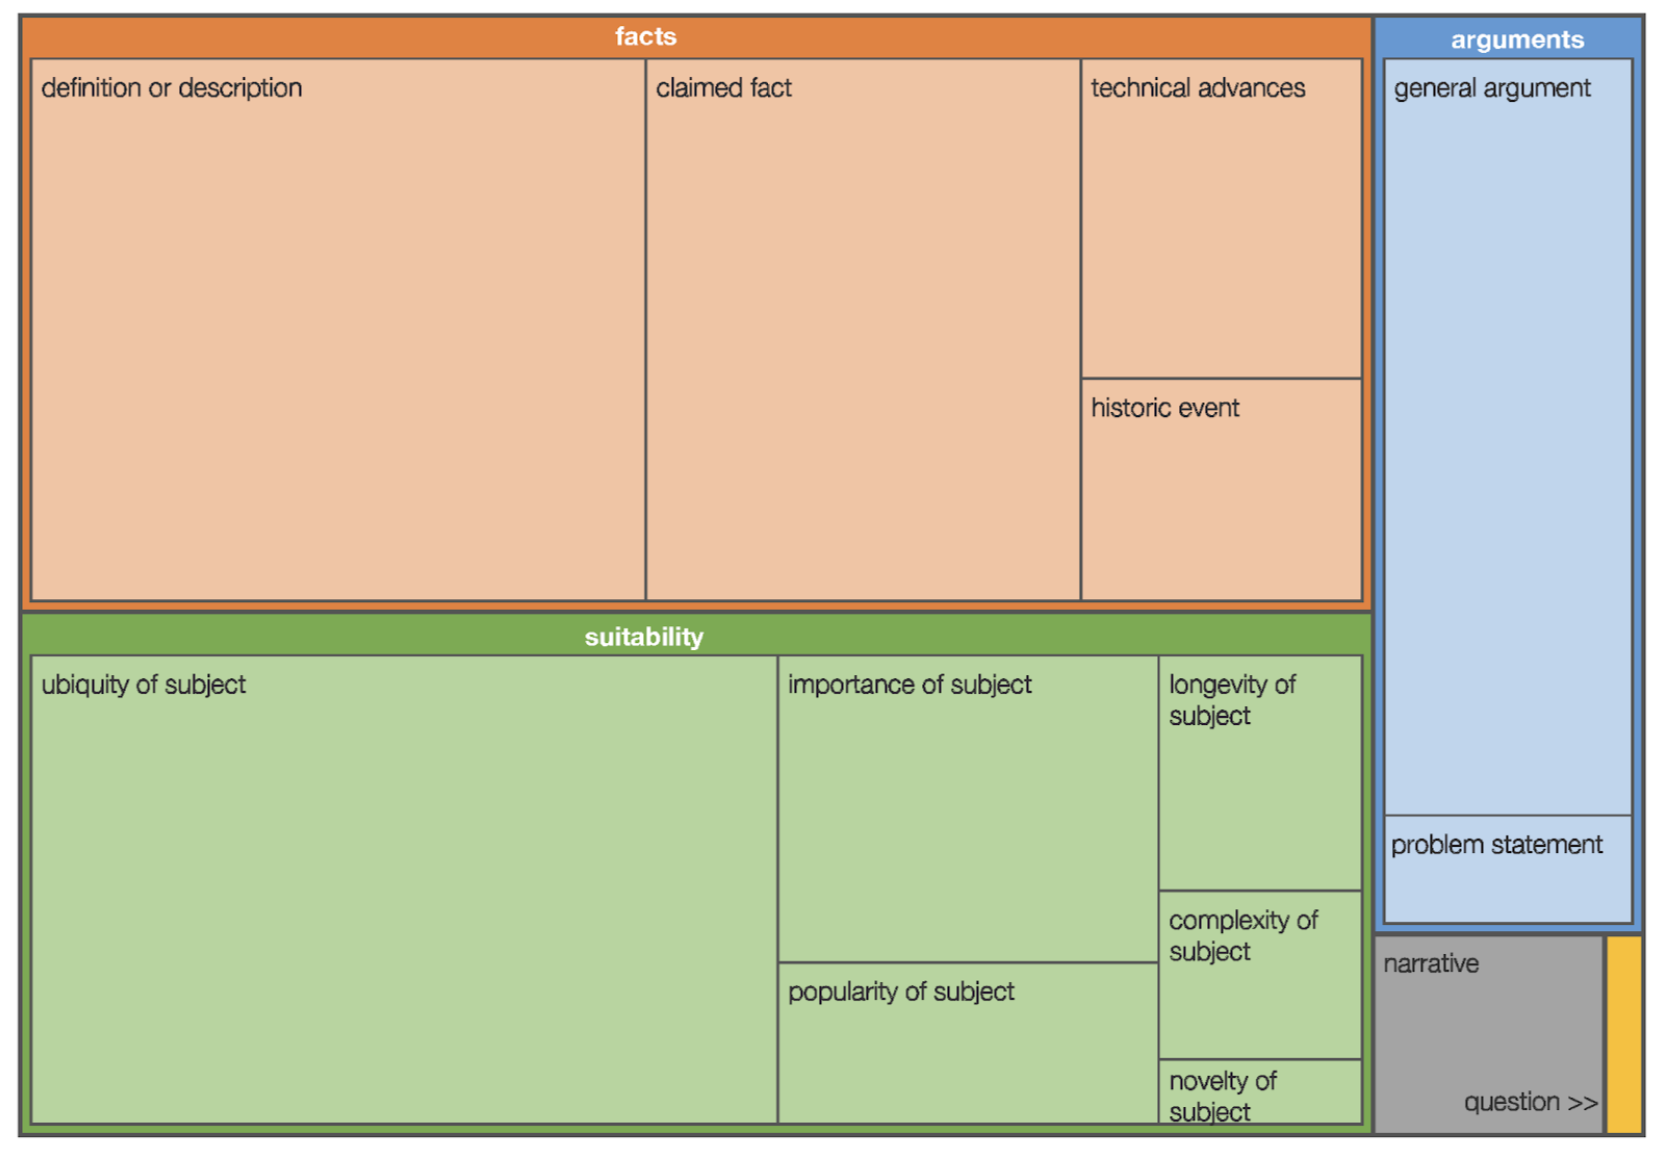
\includegraphics[width=0.5\textwidth]{image.png}
		\caption{Overview of the categorization of opening sentences}
		\label{fig:overview}
	\end{figure*}
	\subsection{Facts}
	\subsubsection{Facts: Definition or Description}
	
	Many papers start with a straightforward definition of the subject of the paper. These tend to be neutral and like something you’d read in a glossary.
	
	``Malware sandboxes are automated dynamic analysis tools that execute samples in an isolated and instrumented environment.''
	
	``Secure two-party computation allows two parties to process their sensitive data in such a way that its privacy is protected.''
	
	``HMAC is a cryptographic authentication algorithm, the ‘Keyed-Hash Message Authentication Code,’ widely used in conjunction with the SHA-256 cryptographic hashing primitive.''
	
	Similarly, papers might provide a description of what the subject of a sentence does or how it works. These are also neutral statements and like something you’d read in a textbook. 
	
	``Traditionally, digital investigations have aimed to recover evidence of a cyber-crime or perform incident response via analysis of non-volatile storage.''
	
	``Mobile social applications discover nearby users and provide services based on user activity (what the user is doing) and context (who and what is nearby).''
	
	``To reduce the memory footprint of a system, the system software shares identical memory pages between processes running on the system.''
	
	\subsubsection{Facts: Claimed Fact}
	
	Another neutral approach to an opening sentence is to provide a fact that is relevant to the subject of the paper. Later we will discuss arguments which are often expressed as if they are facts but are only debatably true. A claimed fact’s correctness should either be apparent or at least provable (i.e., falsifiable). 
	
	``Users are often advised or required to choose passwords that comply with certain policies.''
	
	``Mobile apps frequently demand access to private information.''
	
	``For several decades, car keys have been used to physically secure vehicles.''
	
	``Some sentences use stronger and more vivid language but are still factually based.'' 
	
	``In spite of extensive industrial and academic efforts (e.g., [3, 41, 42]), distributed denial-of-service (DDoS) attacks continue to plague the Internet.''
	
	\subsubsection{Facts: Technical Advances}
	
	Many opening sentences lay out a technical advance in the subject of the sentence. This creates a window of opportunity for the researcher to later identify a novel research problem caused by the changing technology.  It is common to see words like: evolve, become, transition, and improve.
	
	``Recent advances in cloud computing enable customers to outsource their computing tasks to the cloud service providers (CSPs).''
	
	``Browsers have evolved over recent years to mediate a wealth of user interactions with sensitive data.''
	
	``Since its beginning in the early nineties, the Web evolved from a mechanism to publish and link static documents into a sophisticated platform for distributed Web applications.''
	
	\subsubsection{Facts: Historic Events}
	
	A final neutral opening sentence will refer to some historic event. 
	
	``In 1996, Wagner and Schneier performed an analysis of the SSL 3.0 protocol [67].''
	
	``In February 2011, a new Tor hidden service [16], called “Silk Road,” opened its doors.''
	
	``The Network Time Protocol (NTP) is one of the Internet’s oldest protocols, dating back to RFC 958 [15] published in 1985.''
	
	In some cases, a paper opens with a “compound” sentence that makes reference to a historic event in one clause of the sentence, while having additional clauses of a different category. For example, the following sentence refers to a historic event as well as a technical advance.
	
	``Starting from Denning’s seminal work in 1986 [9], intrusion detection has evolved into a number of different approaches.''
	
	\subsection{Arguments}
	\subsubsection{Arguments: General Argument}
	
	Many opening sentences issue a subjective argument that represents the authors’ opinion. Unlike a fact, it isn’t straightforward that the reader will accept it as true. While arguments are less neutral than facts, they can be more interesting and provocative, which can help draw the reader into the paper.
	
	The arguments we categorize under “general arguments” do not fit elsewhere in our categorization system. As we go through more categories, we will see other more specific kinds of arguments. 
	
	``It is a truth universally acknowledged, that password-based authentication on the web is insecure.''
	
	``The dismissal of human memory by the security community reached the point of parody long ago.''
	
	``In recent years, unwanted software has risen to the forefront of threats facing users.''
	
	``The phenomenal growth of Android devices brings in a vibrant application ecosystem.''
	
	\subsubsection{Arguments: Problem Statement }
	
	A special type of argument is a “problem statement” which uses the opening sentence to establish a problem or challenge to be solved. 
	
	``A key challenge when running untrusted virtual machines is providing them with efficient and secure I/O.''
	
	``Determining the semantic similarity between two pieces of binary code is a central problem in a number of security settings.''
	
	``It is difficult to keep secrets during program execution.''
	
	For some sentences, the problem is not stated explicitly but can be inferred from what is said. For example, the “pressure to respond” in the following sentence implies a problem.
	
	``As popular applications rely on personal, privacy-sensitive information about users, factors such as legal regulations, industry self-regulation, and a growing body of privacy-conscious users all pressure developers to respond to demands for privacy.''
	
	\subsection{Suitability}
	\subsubsection{Suitability: Importance of subject}
	
	A large set of sentences make a special kind of argument: that the subject of the opening sentence is suitable or worthy of research. The exact reasons they are suitable fall into a few sub-categories: the subject is important, ubiquitous, complex, novel, popular with other researchers, or has been around a long time. 
	
	Many opening sentences state that their subject is important, with the implication that it is thus suitable for research.
	
	``Security has now become an important and real concern to connected and/or automated vehicles.''
	
	``Error handling is an important aspect of software development.''
	
	``SSL/TLS is, due to its enormous importance, a major target for attacks.''
	
	Some sentences do not explicitly use the word “important” but find other ways to convey the same notion. For example, a concern or component might be described as essential or crucial or serious.
	
	``The threat of data theft in public and private clouds from insiders (e.g. curious administrators) is a serious concern.''
	
	``The same-origin policy (SOP) is a cornerstone of web security, guarding the web content of one domain from the access from another domain."
	
	\subsubsection{Suitability: Ubiquity of subject}
	
	The most popular kind of opening sentence argues that a subject is suitable for research because it is ubiquitous and widely used.
	
	``Billions of users now depend on online services for sensitive communication.''
	
	``Embedded systems are omnipresent in our everyday life.''
	
	``Android is the major platform for mobile users and mobile app developers.''
	
	\subsubsection{Suitability: Popularity of subject}
	
	While the ubiquity of a subject corresponds to how widely it is used, a closely related variant points out that the subject has received a lot of attention. Often, this means attention from other researchers which lends credibility to the subject for further research.
	
	``Protecting the privacy of user data within mobile applications (apps for short) has always been at the spotlight of mobile security research.''
	
	``The black-market economy for purchasing Facebook likes, Twitter followers, and Yelp and Amazon reviews has been widely acknowledged in both industry and academia [6, 27, 37, 58, 59].''
	
	``Since the first widely-exploited buffer overflow used by the 1998 Morris worm [27], the prevention, exploitation, and mitigation of memory corruption vulnerabilities have occupied the time of security researchers and cybercriminals alike.''
	
	\subsubsection{Suitability: Longevity of subject }
	
	In this category, how long a subject has been around is the key component to why it is a suitable subject for study. In some cases, a specific duration is provided and in others, it is implied that the amount of time is significant.
	
	``Redaction of sensitive information from documents has been used since ancient times as a means of concealing and removing secrets from texts intended for public release.''
	
	``Since its beginning in the early nineties, the Web evolved from a mechanism to publish and link static documents into a sophisticated platform for distributed Web applications.''
	
	\subsubsection{Suitability: Complexity of subject}
	
	In this category, the complexity of the subject is highlighted, implying that the complexity creates new issues or requires further research. The complexity might be inherent to the subject itself. Or there might be a complex set of external factors to consider.
	
	``Today, large and complex software is built with many components integrated using APIs.''
	
	``The capabilities and limitations of disassembly are not always clearly defined or understood, making it difficult for researchers and reviewers to judge the practical feasibility of techniques based on it.''
	
	``As popular applications rely on personal, privacy-sensitive information about users, factors such as legal regulations, industry self-regulation, and a growing body of privacy-conscious users all pressure developers to respond to demands for privacy.''
	
	\subsubsection{Suitability: Novelty of subject}
	
	Finally, a degree of novelty is an important component in any research question so it is unsurprising that papers begin arguing novelty from their opening sentence. In this category, sentences focus on something that is new or emerging. 
	
	``In the last few years, a new class of cyber attacks has emerged that is more targeted at individuals and organizations.''
	
	``Although the operating system (OS) kernel has always been an appealing target, until recently attackers focused mostly on the exploitation of vulnerabilities in server and client applications— which often run with administrative privileges—as they are (for the most part) less complex to analyze and easier to compromise.''
	
	``This sentence manages to appeal to both longevity and novelty by relating two subjects.''
	
	``While cryptocurrency has been studied since the 1980s [22, 25, 28], bitcoin is the first to see widespread adoption.''
	
	\subsection{Narrative}
	
	A potentially interesting way to draw a reader into a paper is by establishing a narrative: a scenario that gets the reader thinking about themselves or other people and what they might do.  
	
	``Consider that you are a domain owner, holding a few domain names that you do not have a better use of.''
	
	``Consider the setting where a client owns a public input x, a server owns a private input w, and the client wishes to learn z := F(x,w) for a program F known to both parties.''
	
	``Narratives might also set a scene, like the academic version of an “establishing shot” from films and TV. ''
	
	``Our phones are always within reach and their location is mostly the same as our location.''
	
	``We live in a “big data” world.''
	
	``The battle for the living room is in full swing.''
	
	\subsection{Question} 
	
	Making the reader curious is another good way to begin a paper, and this can be accomplished using a question. In our sample, this was underused with only one example.
	
	``Do programmers leave fingerprints in their source code?''
	
	\section{Conclusion and Future Work}
	
	As researchers, we often find ourselves staring at the blinking cursor, trying to come up with a witty and neat way to start our paper to engage the audience. The opening sentence has a responsibility because it is a way to be remembered, just like in the novels. Chances are high that you recognize many opening sentences of famous literary works even if you haven’t read them. Knowing how many times we have struggled with an opening sentence, we were curious how other researchers begin their papers. We know every researcher has their own style of telling the story of their research process. 
	
	We also discuss whether a similar classification can be used in other domains or the categories that we present in this paper are domain-specific. And if we can use the same categories, how the weights of these categories differ in other areas.
	
	Future work maybe:
	
	In other domains: categories can completely change or same categories can be used but their weights change.
	
	Maybe in history, political science or economics a similar classification can be used?
	
	But we think that we may need different categories if we do the same study in literature. 
	
	
	We also observe that the opening sentences that we coded are not too elaborate or ornate (this type of writing is defined as `purple prose').
	
	
	
	\bibliographystyle{ACM-Reference-Format}
	\bibliography{acmart}
\end{document}
\endinput
%%
%% End of file `sample-sigconf.tex'.
